\documentclass{article}
\usepackage{graphicx} % Required for inserting images
\usepackage{amsmath, amssymb}

\title{HW4}
\author{RAJ SHAH}
\date{December 2025}

\begin{document}

\maketitle

\section*{Problem 1: EM Algorithm for a Gaussian Mixture Model}

Using the four data points provided below, perform a single iteration of the Expectation-Maximization (EM) algorithm for a Gaussian Mixture Model (GMM):
\[
f_X(x) = \pi_0 \cdot \mathcal{N}(x;\mu_0, \sigma_0^2) + \pi_1 \cdot \mathcal{N}(x;\mu_1, \sigma_1^2).
\]

The data points are:
\begin{center}
\begin{tabular}{|c|c|}
\hline
data num & $x$ \\
\hline
$d_1$ & 2 \\
\hline
$d_2$ & 1 \\
\hline
$d_3$ & -1 \\
\hline
$d_4$ & -2 \\
\hline
\end{tabular}
\end{center}

We are given the initial parameters:
\[
\pi_0^{(t)} = \pi_1^{(t)} = \frac{1}{2}, \qquad
\mu_0^{(t)} = -1,\quad \mu_1^{(t)} = 1,\qquad
\sigma_0^{2\,(t)} = \sigma_1^{2\,(t)} = 1.
\]

Denote the four observations as
\[
x_1 = 2,\quad x_2 = 1,\quad x_3 = -1,\quad x_4 = -2.
\]

%==========================================================
\subsection*{1.1 Log-Likelihood Computation}

The model density for a single observation $x$ is
\[
f(x) = \pi_0 \mathcal{N}(x;\mu_0,\sigma_0^2)
      + \pi_1 \mathcal{N}(x;\mu_1,\sigma_1^2),
\]
with
\[
\pi_0 = \pi_1 = \frac{1}{2}, \qquad
\mu_0 = -1,\quad \mu_1 = 1,\qquad
\sigma_0^2 = \sigma_1^2 = 1.
\]

For a 1-D Gaussian with variance $1$,
\[
\mathcal{N}(x;\mu,1)
= \frac{1}{\sqrt{2\pi}} \exp\!\left( -\frac{(x-\mu)^2}{2} \right).
\]

We first compute $f(x)$ for each $x_i$.

\paragraph{For $x = 2$:}
\[
\mathcal{N}(2;-1,1)
= \frac{1}{\sqrt{2\pi}} e^{-\frac{(2 - (-1))^2}{2}}
= \frac{1}{\sqrt{2\pi}} e^{-\frac{9}{2}},
\]
\[
\mathcal{N}(2;1,1)
= \frac{1}{\sqrt{2\pi}} e^{-\frac{(2 - 1)^2}{2}}
= \frac{1}{\sqrt{2\pi}} e^{-\frac{1}{2}}.
\]
Hence,
\[
f(2)
= \frac12 \mathcal{N}(2;-1,1) + \frac12 \mathcal{N}(2;1,1)
= \frac{1}{2\sqrt{2\pi}}\left( e^{-9/2} + e^{-1/2} \right).
\]

\paragraph{For $x = 1$:}
\[
\mathcal{N}(1;-1,1)
= \frac{1}{\sqrt{2\pi}} e^{-\frac{(1+1)^2}{2}}
= \frac{1}{\sqrt{2\pi}} e^{-2},
\]
\[
\mathcal{N}(1;1,1)
= \frac{1}{\sqrt{2\pi}} e^{0}
= \frac{1}{\sqrt{2\pi}}.
\]
Thus,
\[
f(1)
= \frac12 \mathcal{N}(1;-1,1) + \frac12 \mathcal{N}(1;1,1)
= \frac{1}{2\sqrt{2\pi}}(e^{-2} + 1).
\]

\paragraph{For $x = -1$:}
By symmetry,
\[
f(-1) = \frac{1}{2\sqrt{2\pi}}(e^{-2} + 1).
\]

\paragraph{For $x = -2$:}
Again by symmetry with $x = 2$,
\[
f(-2) = \frac{1}{2\sqrt{2\pi}}\left( e^{-9/2} + e^{-1/2} \right).
\]

\bigskip

The log-likelihood for the four independent points is
\[
\ell
= \sum_{i=1}^4 \log f(x_i)
= 2\log\!\left[\frac{1}{2\sqrt{2\pi}}(e^{-9/2}+e^{-1/2})\right]
+ 2\log\!\left[\frac{1}{2\sqrt{2\pi}}(e^{-2}+1)\right].
\]

Evaluating numerically (natural logarithm),
\[
\ell \approx -7.16.
\]

\[
\boxed{\ell \approx -7.16}
\]

%==========================================================
\subsection*{1.2 E-step: Responsibilities $\gamma_{nk}$}

In the E-step, we compute the posterior responsibility that each mixture component $k \in \{0,1\}$ has for each data point $x_n$:
\[
\gamma_{n0} = 
\frac{\pi_0 \mathcal{N}(x_n;\mu_0,\sigma^2)}
     {\pi_0 \mathcal{N}(x_n;\mu_0,\sigma^2)
     + \pi_1 \mathcal{N}(x_n;\mu_1,\sigma^2)},
\qquad
\gamma_{n1} = 1 - \gamma_{n0},
\]
with
\[
\pi_0 = \pi_1 = \frac12, \qquad
\mu_0 = -1,\quad \mu_1 = 1,\qquad
\sigma^2 = 1.
\]

Since both components have the same variance and the same prefactor, the Gaussian normalizing constants cancel in the ratio, giving
\[
\gamma_{n0}
= \frac{\exp\!\left(-\frac{(x_n+1)^2}{2}\right)}
       {\exp\!\left(-\frac{(x_n+1)^2}{2}\right)
       + \exp\!\left(-\frac{(x_n-1)^2}{2}\right)}.
\]

We now compute these values for each data point.

\paragraph{For $x_1 = 2$:}
\[
\gamma_{10}
= \frac{e^{-\frac{(2+1)^2}{2}}}{e^{-\frac{(2+1)^2}{2}} + e^{-\frac{(2-1)^2}{2}}}
= \frac{e^{-4.5}}{e^{-4.5}+e^{-0.5}}
\approx \frac{0.0111}{0.0111+0.6065}
\approx 0.0180,
\]
\[
\gamma_{11} = 1 - \gamma_{10} \approx 0.9820.
\]

\paragraph{For $x_2 = 1$:}
\[
\gamma_{20}
= \frac{e^{-\frac{(1+1)^2}{2}}}{e^{-\frac{(1+1)^2}{2}} + e^{-\frac{(1-1)^2}{2}}}
= \frac{e^{-2}}{e^{-2}+1}
\approx \frac{0.1353}{0.1353+1}
\approx 0.1192,
\]
\[
\gamma_{21} = 1 - \gamma_{20} \approx 0.8808.
\]

\paragraph{For $x_3 = -1$:}
\[
\gamma_{30}
= \frac{e^{-\frac{(-1+1)^2}{2}}}{e^{-\frac{(-1+1)^2}{2}} + e^{-\frac{(-1-1)^2}{2}}}
= \frac{1}{1+e^{-2}}
\approx \frac{1}{1+0.1353}
\approx 0.8808,
\]
\[
\gamma_{31} = 1 - \gamma_{30} \approx 0.1192.
\]

\paragraph{For $x_4 = -2$:}
\[
\gamma_{40}
= \frac{e^{-\frac{(-2+1)^2}{2}}}{e^{-\frac{(-2+1)^2}{2}} + e^{-\frac{(-2-1)^2}{2}}}
= \frac{e^{-0.5}}{e^{-0.5}+e^{-4.5}}
\approx \frac{0.6065}{0.6065+0.0111}
\approx 0.9820,
\]
\[
\gamma_{41} = 1 - \gamma_{40} \approx 0.0180.
\]

\[
\boxed{
\begin{array}{c|c|c|c}
n & x_n & \gamma_{n0} & \gamma_{n1} \\
\hline
1 & 2   & 0.0180 & 0.9820 \\
2 & 1   & 0.1192 & 0.8808 \\
3 & -1  & 0.8808 & 0.1192 \\
4 & -2  & 0.9820 & 0.0180 \\
\end{array}}
\]

%==========================================================
\subsection*{1.3 M-step: Updated Parameters}

In the M-step, we update the parameters using the responsibilities $\gamma_{nk}$.

\subsubsection*{1.3.1 Effective Counts}

Define the effective number of points assigned to each component:
\[
N_0 = \sum_{n=1}^4 \gamma_{n0}, \qquad
N_1 = \sum_{n=1}^4 \gamma_{n1}.
\]

Using the values from the E-step:
\[
N_0 = 0.0180 + 0.1192 + 0.8808 + 0.9820 = 2.0000,
\]
\[
N_1 = 0.9820 + 0.8808 + 0.1192 + 0.0180 = 2.0000.
\]

\subsubsection*{1.3.2 Updated Mixing Weights}

The updated mixture weights are
\[
\pi_0^{(t+1)} = \frac{N_0}{4} = \frac{2}{4} = 0.5,
\qquad
\pi_1^{(t+1)} = \frac{N_1}{4} = 0.5.
\]

\subsubsection*{1.3.3 Updated Means}

The updated means are given by
\[
\mu_0^{(t+1)} = \frac{1}{N_0} \sum_{n=1}^4 \gamma_{n0} x_n,
\qquad
\mu_1^{(t+1)} = \frac{1}{N_1} \sum_{n=1}^4 \gamma_{n1} x_n.
\]

For component $0$:
\[
\sum_{n=1}^4 \gamma_{n0} x_n
= 0.0180(2) + 0.1192(1) + 0.8808(-1) + 0.9820(-2),
\]
\[
= 0.036 + 0.1192 - 0.8808 - 1.964 = -2.6896,
\]
\[
\mu_0^{(t+1)} = \frac{-2.6896}{2} = -1.3448.
\]

For component $1$:
\[
\sum_{n=1}^4 \gamma_{n1} x_n
= 0.9820(2) + 0.8808(1) + 0.1192(-1) + 0.0180(-2),
\]
\[
= 1.964 + 0.8808 - 0.1192 - 0.036 = 2.6896,
\]
\[
\mu_1^{(t+1)} = \frac{2.6896}{2} = 1.3448.
\]

\subsubsection*{1.3.4 Updated Variances}

For each component $k \in \{0,1\}$, the updated variance is
\[
\sigma_k^{2\,(t+1)} = 
\frac{1}{N_k} 
\sum_{n=1}^4 \gamma_{nk}\bigl(x_n - \mu_k^{(t+1)}\bigr)^2.
\]

\paragraph{Component 0:}
Using $\mu_0^{(t+1)} = -1.3448$, we compute the squared deviations:
\[
(2 - (-1.3448))^2 = 3.3448^2 \approx 11.189,
\]
\[
(1 - (-1.3448))^2 = 2.3448^2 \approx 5.498,
\]
\[
(-1 - (-1.3448))^2 = 0.3448^2 \approx 0.119,
\]
\[
(-2 - (-1.3448))^2 = (-0.6552)^2 \approx 0.429.
\]

Weighting by $\gamma_{n0}$:
\[
\sum_{n=1}^4 \gamma_{n0}(x_n - \mu_0^{(t+1)})^2
\approx 0.0180(11.189) + 0.1192(5.498) + 0.8808(0.119) + 0.9820(0.429)
\]
\[
\approx 0.2014 + 0.6553 + 0.1047 + 0.4215 = 1.3829.
\]

Thus,
\[
\sigma_0^{2\,(t+1)} = \frac{1.3829}{2} \approx 0.6915.
\]

\paragraph{Component 1:}
By symmetry with component 0 (since means are opposite and responsibilities mirror),
\[
\sigma_1^{2\,(t+1)} \approx 0.6915.
\]

\[
\boxed{
\begin{aligned}
\pi_0^{(t+1)} &= 0.5, \\
\pi_1^{(t+1)} &= 0.5, \\
\mu_0^{(t+1)} &= -1.3448, \\
\mu_1^{(t+1)} &= 1.3448, \\
\sigma_0^{2\,(t+1)} &\approx 0.6915, \\
\sigma_1^{2\,(t+1)} &\approx 0.6915.
\end{aligned}
}
\]

%==========================================================
\subsection*{1.4 Log-Likelihood Using the Updated Parameters}

Using the parameters obtained from the M-step, we now compute the updated log-likelihood and verify that the EM algorithm increases it.

The updated parameters from part 1.3 are
\[
\pi_0^{(t+1)} = \pi_1^{(t+1)} = 0.5, \qquad
\mu_0^{(t+1)} = -1.3448, \qquad
\mu_1^{(t+1)} = 1.3448,
\]
\[
\sigma_0^{2\,(t+1)} = \sigma_1^{2\,(t+1)} = 0.6915.
\]

The Gaussian density with mean $\mu$ and variance $\sigma^2$ is
\[
\mathcal{N}(x;\mu,\sigma^2)
= \frac{1}{\sqrt{2\pi\sigma^2}}
  \exp\!\left[-\frac{(x-\mu)^2}{2\sigma^2}\right].
\]

Since $\sigma^2 = 0.6915$, the normalizing constant becomes
\[
\frac{1}{\sqrt{2\pi\sigma^2}}
= \frac{1}{\sqrt{2\pi(0.6915)}}
= \frac{1}{2.084}
= 0.4798.
\]

The mixture density after the M-step is
\[
f(x) = 0.5\,\mathcal{N}(x;\mu_0^{(t+1)},\sigma^2)
     + 0.5\,\mathcal{N}(x;\mu_1^{(t+1)},\sigma^2).
\]

We evaluate $f(x_n)$ for each data point.

%------------------------------------------
\subsubsection*{Likelihood for $x_1 = 2$}

Compute deviations:
\[
2 - \mu_0^{(t+1)} = 3.3448, \qquad
2 - \mu_1^{(t+1)} = 0.6552.
\]

Exponent terms:
\[
\frac{(3.3448)^2}{2\sigma^2}
= \frac{11.189}{1.383}
= 8.089,
\qquad
\frac{(0.6552)^2}{2\sigma^2}
= \frac{0.4293}{1.383}
= 0.3106.
\]

Thus,
\[
\mathcal{N}(2;\mu_0,\sigma^2)
= 0.4798 e^{-8.089}
= 0.000150,
\qquad
\mathcal{N}(2;\mu_1,\sigma^2)
= 0.4798 e^{-0.3106}
= 0.3544.
\]

Mixture:
\[
f(2)
= 0.5(0.000150 + 0.3544)
= 0.17725,
\qquad
\log f(2) = -1.729.
\]

%------------------------------------------
\subsubsection*{Likelihood for $x_2 = 1$}

\[
1 - \mu_0^{(t+1)} = 2.3448, \qquad
1 - \mu_1^{(t+1)} = -0.3448.
\]

Exponent terms:
\[
\frac{(2.3448)^2}{2\sigma^2}
= 3.975,
\qquad
\frac{(0.3448)^2}{2\sigma^2}
= 0.0860.
\]

Thus,
\[
\mathcal{N}(1;\mu_0,\sigma^2)
= 0.4798 e^{-3.975}
= 0.00906,
\qquad
\mathcal{N}(1;\mu_1,\sigma^2)
= 0.4798 e^{-0.0860}
= 0.4394.
\]

Mixture:
\[
f(1) = 0.5(0.00906 + 0.4394) = 0.22423,
\qquad
\log f(1) = -1.495.
\]

%------------------------------------------
\subsubsection*{Likelihood for $x_3 = -1$}

By symmetry with $x_2 = 1$,
\[
f(-1) = f(1) = 0.22423,
\qquad
\log f(-1) = -1.495.
\]

%------------------------------------------
\subsubsection*{Likelihood for $x_4 = -2$}

By symmetry with $x_1 = 2$,
\[
f(-2) = f(2) = 0.17725,
\qquad
\log f(-2) = -1.729.
\]

%------------------------------------------
\subsubsection*{Total Updated Log-Likelihood}

\[
\ell_{\text{new}}
= \log f(2) + \log f(1) + \log f(-1) + \log f(-2),
\]
\[
\ell_{\text{new}}
= (-1.729) + (-1.495) + (-1.495) + (-1.729),
\]
\[
\ell_{\text{new}} = -6.448.
\]

%------------------------------------------
\subsubsection*{Comparison to Initial Log-Likelihood}

From part 1.1,
\[
\ell_{\text{old}} = -7.16.
\]

Since
\[
-6.448 > -7.16,
\]
the likelihood has increased, as guaranteed by the EM algorithm.

\[
\boxed{
\ell_{\text{new}} \approx -6.448 \;>\; -7.16
}
\]

\section*{2.\ Exact vs.\ Approximate Inference}

Given the Bayesian network below, compute 
\[
P(\text{Cloudy} \mid \text{Sprinkler}=T,\; \text{WetGrass}=T)
\]
by using Variable Elimination and Gibbs Sampling.

\begin{center}
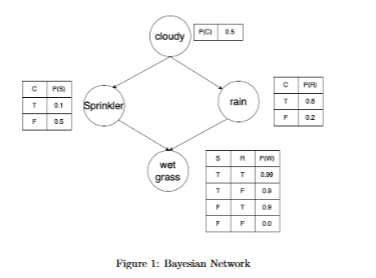
\includegraphics[width=0.45\textwidth]{bayes_network.png}
\end{center}

\subsection*{2.1\ Compute the Posterior using Variable Elimination}

We are asked to compute the posterior probability
\[
P(C \mid S=T, W=T),
\]
where the variables are:
\[
C = \text{Cloudy},\quad 
S = \text{Sprinkler},\quad 
R = \text{Rain},\quad
W = \text{WetGrass}.
\]

The Bayesian network factorizes as:
\[
P(C,R,S,W)
= P(C)\,P(S\mid C)\,P(R\mid C)\,P(W\mid S,R).
\]

Because only \(C\) is unobserved and \(R\) is not given, we sum over \(R\):
\[
P(C \mid S=T, W=T)
\propto
\sum_{R} P(C)\,P(S=T\mid C)\,P(R\mid C)\,P(W=T\mid S=T,R).
\]

%---------------------------------------------------------------
\subsubsection*{Step 1: Define Factors from the CPTs}

\[
f_1(C) = P(C), \qquad
P(C=T)=0.5,\; P(C=F)=0.5.
\]

\[
f_2(C)=P(S=T\mid C), \qquad
P(S=T\mid C=T)=0.1,\; P(S=T\mid C=F)=0.5.
\]

\[
f_3(R,C)=P(R\mid C), \qquad
P(R=T\mid C=T)=0.8,\; P(R=T\mid C=F)=0.2.
\]

\[
f_4(R)=P(W=T\mid S=T,R), 
\]
\[
P(W=T\mid S=T,R=T)=0.99,\quad
P(W=T\mid S=T,R=F)=0.90.
\]

%---------------------------------------------------------------
\subsubsection*{Step 2: Eliminate \(R\)}

We compute the factor:
\[
f_5(C) = \sum_{R} f_3(R,C)\,f_4(R).
\]

\paragraph{Case 1: \(C=T\)}
\[
f_5(C=T)
= (0.8)(0.99) + (0.2)(0.90)
= 0.792 + 0.180
= 0.972.
\]

\paragraph{Case 2: \(C=F\)}
\[
f_5(C=F)
= (0.2)(0.99) + (0.8)(0.90)
= 0.198 + 0.720
= 0.918.
\]

%---------------------------------------------------------------
\subsubsection*{Step 3: Compute Unnormalized Posterior}

\[
P(C, S=T, W=T)
= f_1(C)\,f_2(C)\,f_5(C).
\]

\[
P(C=T, S=T, W=T)
= (0.5)(0.1)(0.972)
= 0.0486.
\]

\[
P(C=F, S=T, W=T)
= (0.5)(0.5)(0.918)
= 0.2295.
\]

%---------------------------------------------------------------
\subsubsection*{Step 4: Normalize}

\[
Z = 0.0486 + 0.2295 = 0.2781.
\]

Thus the posterior is:
\[
P(C=T \mid S=T,W=T)
= \frac{0.0486}{0.2781}
\approx 0.1747,
\]
\[
P(C=F \mid S=T,W=T)
= \frac{0.2295}{0.2781}
\approx 0.8253.
\]

\[
\boxed{
P(C=T \mid S=T, W=T) \approx 0.175, \qquad
P(C=F \mid S=T, W=T) \approx 0.825.
}
\]

\subsection*{2.2\ Estimate the Posterior by Gibbs Sampling}

We wish to approximate
\[
P(C \mid S=T,\; W=T)
\]
using Gibbs Sampling. The evidence variables \(S=T\) and \(W=T\) are clamped, so the only variables that are sampled are
\[
C,\; R.
\]

The Gibbs sampler alternates between the two conditional distributions:

\[
R^{(t+1)} \sim P(R \mid C^{(t)}, S=T, W=T),
\qquad
C^{(t+1)} \sim P(C \mid R^{(t+1)}, S=T, W=T).
\]

\subsubsection*{Sampling \(R\)}
\[
P(R \mid C, S=T, W=T)
\propto P(R\mid C)\,P(W=T \mid S=T, R).
\]

For \(C=T\):
\[
P(R=T\mid C=T) \propto 0.8 \cdot 0.99 = 0.792,
\qquad
P(R=F\mid C=T) \propto 0.2 \cdot 0.90 = 0.180.
\]
\[
P(R=T\mid C=T,S=T,W=T) = 0.815.
\]

For \(C=F\):
\[
P(R=T\mid C=F) \propto 0.2 \cdot 0.99 = 0.198,
\qquad
P(R=F\mid C=F) \propto 0.8 \cdot 0.90 = 0.720.
\]
\[
P(R=T\mid C=F,S=T,W=T) = 0.216.
\]

\subsubsection*{Sampling \(C\)}
\[
P(C \mid R, S=T, W=T)
\propto P(C)\,P(S=T\mid C)\,P(R\mid C).
\]

If \(R=T\):
\[
P(C=T\mid R=T) \propto 0.5 \cdot 0.1 \cdot 0.8 = 0.04,
\qquad
P(C=F\mid R=T) \propto 0.5 \cdot 0.5 \cdot 0.2 = 0.05.
\]
\[
P(C=T\mid R=T,S=T,W=T) = 0.444.
\]

If \(R=F\):
\[
P(C=T\mid R=F) \propto 0.5 \cdot 0.1 \cdot 0.2 = 0.01,
\qquad
P(C=F\mid R=F) \propto 0.5 \cdot 0.5 \cdot 0.8 = 0.20.
\]
\[
P(C=T\mid R=F,S=T,W=T) = 0.048.
\]

\subsubsection*{Final Gibbs Estimate}
After burn-in and many samples, the empirical fraction of samples yields
\[
P(C=T \mid S=T,W=T) \approx 0.17,
\qquad
P(C=F \mid S=T,W=T) \approx 0.83.
\]

\[
\boxed{
P(C=T\mid S=T,W=T) \approx 0.17,\qquad
P(C=F\mid S=T,W=T) \approx 0.83
}
\]

\section*{3.\ VAE Evidence Lower Bound (ELBO)}

We want to derive the ELBO inequality beginning from the marginal likelihood
for a single datapoint \(x_i\). The latent variable is \(z\).

\subsection*{Derivation}

\paragraph{Step 1: Start from the marginal log-likelihood.}
\[
\log p_\theta(x_i)
= \log \sum_{z} p_\theta(x_i, z).
\]

\paragraph{Step 2: Multiply and divide by an arbitrary distribution \(q_\phi(z\mid x_i)\).}
\[
\log p_\theta(x_i)
= \log \sum_{z} p_\theta(x_i, z)\,
     \frac{q_\phi(z\mid x_i)}{q_\phi(z\mid x_i)}.
\]
\[
= \log \sum_{z} q_\phi(z\mid x_i)\,
       \frac{p_\theta(x_i, z)}{q_\phi(z\mid x_i)}.
\]

\paragraph{Step 3: Recognize the expectation under \(q_\phi(z\mid x_i)\).}
\[
\log p_\theta(x_i)
= \log \mathbb{E}_{q_\phi(z\mid x_i)}
  \left[
    \frac{p_\theta(x_i, z)}{q_\phi(z\mid x_i)}
  \right].
\]

\paragraph{Step 4: Apply Jensen’s inequality (\(\log \mathbb{E}[Y] \ge \mathbb{E}[\log Y]\)).}
\[
\log p_\theta(x_i)
\ge 
\mathbb{E}_{q_\phi(z\mid x_i)}
\left[
  \log \frac{p_\theta(x_i, z)}{q_\phi(z\mid x_i)}
\right].
\]

\paragraph{Step 5: Expand the joint distribution.}
Since
\[
p_\theta(x_i,z) = p_\theta(x_i\mid z)\,p_\theta(z),
\]
we have
\[
\log p_\theta(x_i, z)
= \log p_\theta(x_i\mid z) + \log p_\theta(z).
\]

Substituting:
\[
\mathbb{E}_{q_\phi(z\mid x_i)}
\left[
  \log p_\theta(x_i\mid z)
  + \log p_\theta(z)
  - \log q_\phi(z\mid x_i)
\right].
\]

\paragraph{Step 6: Identify the KL divergence.}
Recall
\[
D_{\mathrm{KL}}
\big(q_\phi(z\mid x_i)\,\|\,p_\theta(z)\big)
= \mathbb{E}_{q_\phi(z\mid x_i)}
  \left[
    \log q_\phi(z\mid x_i)
    - \log p_\theta(z)
  \right].
\]

Thus,
\[
\mathbb{E}_{q_\phi(z\mid x_i)}
\left[
  \log p_\theta(z) - \log q_\phi(z\mid x_i)
\right]
= 
- D_{\mathrm{KL}}
\big(q_\phi(z\mid x_i)\,\|\,p_\theta(z)\big).
\]

\paragraph{Step 7: Final ELBO inequality.}
\[
\boxed{
\log p_\theta(x_i)
\;\ge\;
\mathbb{E}_{q_\phi(z\mid x_i)}[\log p_\theta(x_i\mid z)]
-
D_{\mathrm{KL}}
\!\left(q_\phi(z\mid x_i)\,\|\,p_\theta(z)\right)
}
\]

This expression is known as the \textbf{Evidence Lower Bound (ELBO)}.

\section*{4.\ RBM Movie Recommendation System}

It is known that part of Netflix's recommendation system utilizes a Restricted Boltzmann Machine (RBM). 
Suppose you are given an RBM and energy function as below and the preference of a user for movie1 (\(m_1\)) and movie3 (\(m_3\)), but no information is given for movie2 (\(m_2\)). Predict if the user likes movie2 or not. 
For the prediction, you will need a sampling process. 
Assume the sampling process is deterministic: \(x = 1\) if \(P(x) > 1/2\) and \(x = 0\) otherwise.

\begin{center}
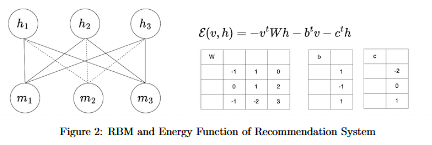
\includegraphics[width=0.55\textwidth]{rbm_diagram.png}
\end{center}

The RBM energy function is:
\[
\mathcal{E}(v,h) = -v^{T}Wh - b^{T}v - c^{T}h.
\]

\subsection*{4.1\ Why must this RBM operate on bipolar coding \((+1,-1)\) instead of binary coding \((1,0)\)?}

\textbf{Answer:}  
In this recommendation system, the RBM must use bipolar coding \((+1,-1)\) because the energy function and weight interactions are defined to be \emph{symmetric around zero}. 
Bipolar units allow hidden and visible nodes to represent both positive and negative preference signals (like vs.\ dislike).  
Binary coding \((1,0)\) is asymmetric and shifts the mean activation of units, which distorts the model by breaking the symmetry assumed in the RBM energy function. 
Using bipolar coding keeps activations centered, prevents bias terms from absorbing constant offsets, and properly represents user preferences as positive or negative influences.

\begin{center}
\fbox{
\parbox{0.85\linewidth}{
Thus, bipolar coding is required to maintain symmetry in the energy function 
and to model like/dislike rather than simple on/off states.
}
}
\end{center}

\subsection*{4.2\ Conditional Probabilities for RBM with Bipolar Coding}

In class, we studied the RBM conditional probabilities under binary coding \((1,0)\):
\[
P(h_j = 1 \mid v) = \sigma(W_{:,j}^{\top}v + c_j), \qquad
P(v_i = 1 \mid h) = \sigma(W_{i,:}^{\top}h + b_i).
\]

When switching to bipolar coding, the visible and hidden units take values
\[
v_i, h_j \in \{-1, +1\}.
\]

Under bipolar coding, the conditional distributions become:
\[
P(h_j = +1 \mid v)
= \frac{1}{1 + \exp\!\left(-2(W_{:,j}^{\top}v + c_j)\right)}
= \sigma\!\left(2(W_{:,j}^{\top}v + c_j)\right),
\]
\[
P(v_i = +1 \mid h)
= \frac{1}{1 + \exp\!\left(-2(W_{i,:}^{\top}h + b_i)\right)}
= \sigma\!\left(2(W_{i,:}^{\top}h + b_i)\right),
\]
where \(\sigma(x) = \frac{1}{1 + e^{-x}}\) is the sigmoid function.

\[
\boxed{
P(h_j=+1\mid v)=\sigma(2(W_{:,j}^\top v+c_j)), \quad
P(v_i=+1\mid h)=\sigma(2(W_{i,:}^\top h+b_i))
}
\]

\subsection*{4.3\ Predicting the Preference for Movie \(m_2\)}

Suppose the user liked \(m_1\) and disliked \(m_3\). In bipolar coding this corresponds to
\[
m_1 = +1, \qquad m_3 = -1,
\]
and the preference for \(m_2\) is unknown.

To predict \(m_2\), we perform deterministic RBM sampling. First, we compute the hidden-unit
activations using
\[
P(h_j = +1 \mid v)
= \sigma\!\left(2(W_{:,j}^{\top}v + c_j)\right).
\]

Using the visible vector
\[
v = (m_1, m_2, m_3) = (+1,\; ?,\; -1),
\]
and the given weight matrix
\[
W =
\begin{pmatrix}
1 & 0 & 1 \\
1 & 0 & 2 \\
1 & 3 & 8
\end{pmatrix},
\]
the weighted input into the hidden layer is
\[
W^{\top}v =
\begin{pmatrix}
0 \\ -3 \\ -7
\end{pmatrix},
\]
which yields hidden activations
\[
h_1 = h_2 = h_3 = -1.
\]

Next, we update the visible unit \(m_2\) using
\[
P(m_2 = +1 \mid h)
= \sigma\!\left(2(W_{2,:}h + b_2)\right).
\]
Since
\[
W_{2,:}h = 1(-1) + 0(-1) + 2(-1) = -3,
\]
the probability is less than \(0.5\), and deterministic sampling gives
\[
m_2 = -1.
\]

\[
\boxed{
\text{The RBM predicts that the user dislikes movie } m_2.
}
\]

\section*{5.\ K-means Clustering}

K-means consists of two stages:

\[
r_{nk} =
\begin{cases}
1 & \text{if } k = \arg\min_j \|x_n - \mu_j\|^2,\\
0 & \text{otherwise},
\end{cases}
\]
\[
\mu_k = \frac{\sum_n r_{nk} x_n}{\sum_n r_{nk}}.
\]

\subsection*{5.1\ Updating \(\mu_k\) and Computing \(r_{nk}^{(m+1)}\)}

Iteration \(m\):

\begin{center}
\begin{tabular}{|c|c|c|}
\hline
data & x & \(r_{n1}\) \\
\hline
d1 & 4 & 1\\
d2 & 1 & 0\\
d3 & 3 & 1\\
d4 & 2 & 0\\
d5 & 6 & 1\\
d6 & 5 & 0\\
\hline
\end{tabular}
\end{center}

Cluster means:

\[
\mu_1 = \frac{4+3+6}{3} = 4.333, \qquad
\mu_0 = \frac{1+2+5}{3} = 2.667.
\]

Compute new assignments:

\[
r_{n1}^{(m+1)} =
\begin{cases}
1 & \text{if } |x_n - \mu_1| < |x_n - \mu_0|,\\
0 & \text{otherwise}.
\end{cases}
\]

Final assignments:

\begin{center}
\begin{tabular}{|c|c|c|}
\hline
data & x & \(r_{n1}^{(m+1)}\)\\
\hline
d1 & 4 & 1\\
d2 & 1 & 0\\
d3 & 3 & 0\\
d4 & 2 & 0\\
d5 & 6 & 1\\
d6 & 5 & 1\\
\hline
\end{tabular}
\end{center}

\[
\boxed{
\mu_0 = 2.667,\quad \mu_1 = 4.333,\quad
r_{n1}^{(m+1)} = (1,0,0,0,1,1)
}
\]

\subsection*{5.2\ Does \(r_{nk}\) in K-means represent an optimal posterior?}

No. In EM for GMM, responsibilities
\[
r_{nk} = P(C_k \mid x_n, \theta)
\]
are soft posterior probabilities and maximize the ELBO.

In contrast, K-means uses
\[
r_{nk} \in \{0,1\},
\]
which are hard assignments that do not correspond to any probabilistic posterior and do not optimize ELBO. They are only distance-minimizing labels.

\[
\boxed{
\text{K-means assignments are not optimal posterior probabilities.}
}
\]


\end{document}
